\subsection{Installing modified classes}
\label{sec:loading}

At a DSU safe point, \JV begins the update by
loading and installing the changed classes, and updating relevant
metadata in the existing versions.

\begin{figure}[t]
\centering
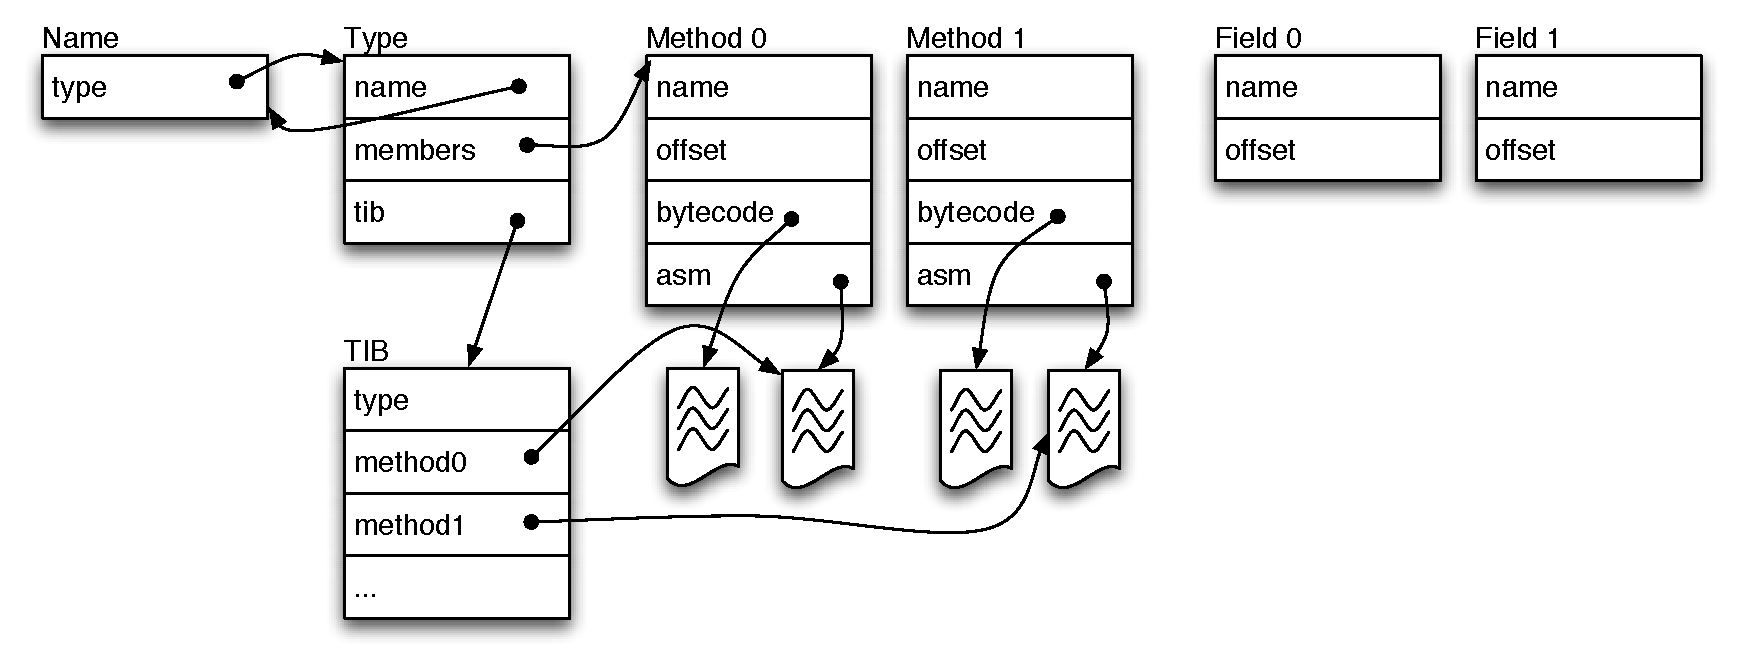
\includegraphics[scale=0.46]{100-images/vm-meta-data}
\hangcaption{\RVM meta-data schema for each class\label{fig:vm-meta-data}}
\VspaceFixForHangcaption
\end{figure}

\begin{figure}[t]
\centering
\includegraphics[scale=0.46]{100-images/vm-meta-data-updated-class}
\hangcaption{\RVM meta-data showing the old class name pointing to a newer
class after an update\label{fig:vm-meta-data-updated-classk}}
\VspaceFixForHangcaption
\end{figure}

\RVM represents classes with several internal data structures.
Figure~\ref{fig:vm-meta-data} shows the information \RVM associates
with a class.  Each class has an \VMClass meta-object that describes the
class. It points to other meta-objects that describe the class's method and
field types and offsets in an object instance.  The compiler and garbage
collector query this metadata. The compiler hard codes these offsets in
generated machine code when accessing fields and when calling methods.
These offsets are statically known when a class is loaded. \RVM and other
\VM{}s lay out fields and methods in \acfp{VMT} in such a way that a given
field or method has the same offset or slot in all subclasses. As explained
in Section~\ref{sec:dsu-view-of-changes}, in \acsp{VMT}, subclass methods
share the same slot as superclass methods they override. This sharing eases
\emph{dynamic dispatch} --- which method is called is decided at
runtime based on the object in hand. When a program invokes a method on an
object, the generated code indexes the object's \VMT at the correct offset
and jumps to the machine code. \RVM uses an array called the \acf{TIB} for
its \VMT. The first entry of the array points to the \VMClass meta-object
for that class. The garbage collector uses this entry to look up the type of a
particular object. The rest of the entries in the array serve as \VMT
slots.

For a class with only method body updates, all of the class's metadata is
the same in both the old and new versions. Therefore, \JV invalidates the
\TIB code entries for each replaced method, reads in the new method body
bytecode, and modifies the existing class metadata to refer to the
replacement methods' bytecode. The \JIT will compile the updated method
when the program next invokes it, after the update.

For a class with changed signature, the class's number, type, and order of
fields or methods may have changed, which in turn impacts the class's
metadata, including its \TIB. \JV modifies existing class metadata as
follows.  First, it changes the old class's metadata to use a modified
class name, e.g., metadata for class \User is renamed to \oUser in our
example update from Figure~\ref{fig:jes-string-emailaddress-example}
and~\ref{fig:jes-transformer-code}. At this point, it is as if {\tt class}
\User never existed. \JV reads in \User's class file as it normally does
and sets up metadata for the new version and updates its data structures
% (e.g., the Java Table of Contents for \static methods and fields)
to indicate that the newly-loaded class is now the up-to-date version.
Note that all \TIB entries for the newly-installed class are invalid, so
all methods in the class will be compiled on demand. \JV invalidates the
\TIB entries and other data structures for the old class so that they can
be garbage-collected.

Invalidating changed methods will impose overhead on the execution just
following the update when these methods are first \emph{base}-compiled and
then when they are progressively optimized at higher levels, if they
execute frequently. We could reduce this overhead somewhat by optimizing
new versions directly to their prior level of optimization. Updates to
method bodies however invalidate execution profiles and  without branch and
call frequencies, code quality would degrade. Thus, we believe it is better
to let the adaptive compiler work as it was intended. In any case, since
dynamic updates are relatively rare events, any added overhead due to
recompilation will be short-lived.

As mentioned in Section~\ref{sec:osr}, \JV uses on-stack replacement to
update active category~(2) methods. The VM triggers on-stack replacement
after the application resumes execution when callees of category~(2)
methods return. In order to resume execution, \JV must update data in the
heap. \JV initiates a full-heap garbage collection and transforms objects of
updated classes, which we get to next.
